% !TEX encoding = UTF-8
% !TEX TS-program = pdflatex
% !TEX root = ../tesi.tex

\chapter{Introduction}
	In this chapter I will describe the tools and softwares I have utilized to carry out the simulations.
	
	\section{Radio Propagation Models}
		A \gls{rpma} is an empirical mathematical formulation used to model the propagation of radio waves as a function of frequency, distance, transmission power and other variables. Over the years various RPMs have been developed, some aiming at modelling a general situation, and others more useful in specific scenarios. For example, implementations range from the more general free space model, where only distance and power are considered, to more complex models which account for shadowing, reflection, scattering and other multipath losses. Moreover, it is important to keep into consideration the computational complexity and scalability of the model: some have poor accuracy but are scalable, while others have very good accuracy but can only work for small sets of nodes. As always, it is very important to find the right tradeoff between complexity and accuracy.
		
		
		The authors of \cite{6298165} classify the propagation models offered by the network simulator ns-3 in three different categories:
		\begin{itemize}
			\item \textbf{Abstract} propagation loss models, for example the Maximal Range model (also known as Unit Disk), which establishes that all transmissions within a certain range are all received without any loss;
			\item \textbf{Deterministic} path loss models, such as the Friis propagation model, which models quadratic path loss as it occurs in free space, and Two Ray Ground, which assume propagation via two rays: a direct (\acrshort{losa}) one, and the one reflected by the ground;
			\item \textbf{Stochastic} fading models such as the Nakagami model, which uses stochastic distributions to model path loss.
		\end{itemize}
	
	
		These traditional models, especially the stochastic ones, work quite well to describe the wireless channel characteristics from a macroscopic point of view. However, given the probabilistic nature of the model, single transmissions are not affected by the mesoscopic and microscopic effects of the sorrounding environment. To keep these effects into consideration, researchers have utilized Ray-Tracing, a geometrical optics technique used to determine all possible signal paths between the transmitter and the receiver, considering reflection, diffraction and scattering of radio waves, suitable both for 2D and 3D scenarios \cite{245274} \cite{765022}.
		
		
		However, a Ray-Tracing based approach, while producing a fairly accurate model, is not very scalable due to its high computational complexity, especially in a real-time scenario. To overcome this problem, the authors of \cite{STEPANOV200861} have resorted to a fairly computationally expensive pre-processing, but this leads to the need of pre-processing every scenario (and also every change in the scenario).
		
		
	
	\section{Obstacle Shadowing propagation loss model}
		The original thesis \cite{ROM2017}, after having analyzed various works concerning shadowing in urban scenarios \cite{Giordano:2010:CST:1860058.1860065} \cite{4020783} used a deterministic \gls{rpma} called Obstacle Shadowing propagation loss model presented in \cite{5720204} and implemented by the authors of \cite{Carpenter:2015:OMI:2756509.2756512}.  This propagation model calculates the loss in signal strength due to the shadowing effect of obstacles such as buildings. 
		
		
		The authors of \cite{5720204} designed the model as an extension of well-established fading models, which can be expressed by Equation \ref{eq:fading-models}, where:
		\begin{itemize}
			\item $P$ are the transmit or receive powers of the radios;
			\item $G$ are the antenna gains;
			\item $L$ indicate the terms capturing loss effects during transmission.
		\end{itemize}
		
		\begin{gather}
			P_r[dBm] = P_t[dBm] + G_t[dB] + G_r[dB] - \sum L_x[dB] 														\label{eq:fading-models}
		\end{gather}
	
		Common RPMs can be written as components L of \ref{eq:fading-models} and chained to obtain the compound attenuation. For example, Equation \ref{eq:tworayground-model} and \ref{eq:lognorm-model} represent respectively the Two-Ray Ground and Log-Normal models.

		\begin{gather}
			L_{TwoRayGround} = 10 \lg \left( \frac{d^4 L}{h^2_t h^2_t} \right)	\qquad [dB]		\label{eq:tworayground-model} \\
			L_{LogNorm} = 10 \lg \left( X_\sigma \right)	\qquad [dB]													\label{eq:lognorm-model}
		\end{gather}
		
		The authors extended the general model shown in \ref{eq:fading-models} adding a $L_{obs}$ term for each obstacle in the line of sight between sender and receiver. The term is described by Equation \ref{eq:osbtacle-model}, where:
		\begin{itemize}
			\item $n$ is the number of times that the line of sight intersects the borders of the obstacle;
			\item $d_m$ is the length of the obstacle's intersections;
			\item $\beta$ represents the attenuation due to the exterior wall of a building, in dB per wall;
			\item $\gamma$ represents an approximation of the internal structure of a building.
		\end{itemize}
		
		
		Parameters $\beta$ and $\gamma$ can be fitted to represent different types of buildings. $\beta \approx$ 9.6 dB per wall and $\gamma \approx$ 0.4 dB/m are the values proposed by the authors for buildings in suburban areas.
		
		\begin{gather}\label{eq:osbtacle-model}
			L_{obs} = \beta n + \gamma d_m
		\end{gather}
	
	
		\imgrefcap{fig:sumo-obstacle} shows an example of transmission where the signal encounters $n =$ 4 walls. 
	
		\begin{figure}[H]
			\centering
			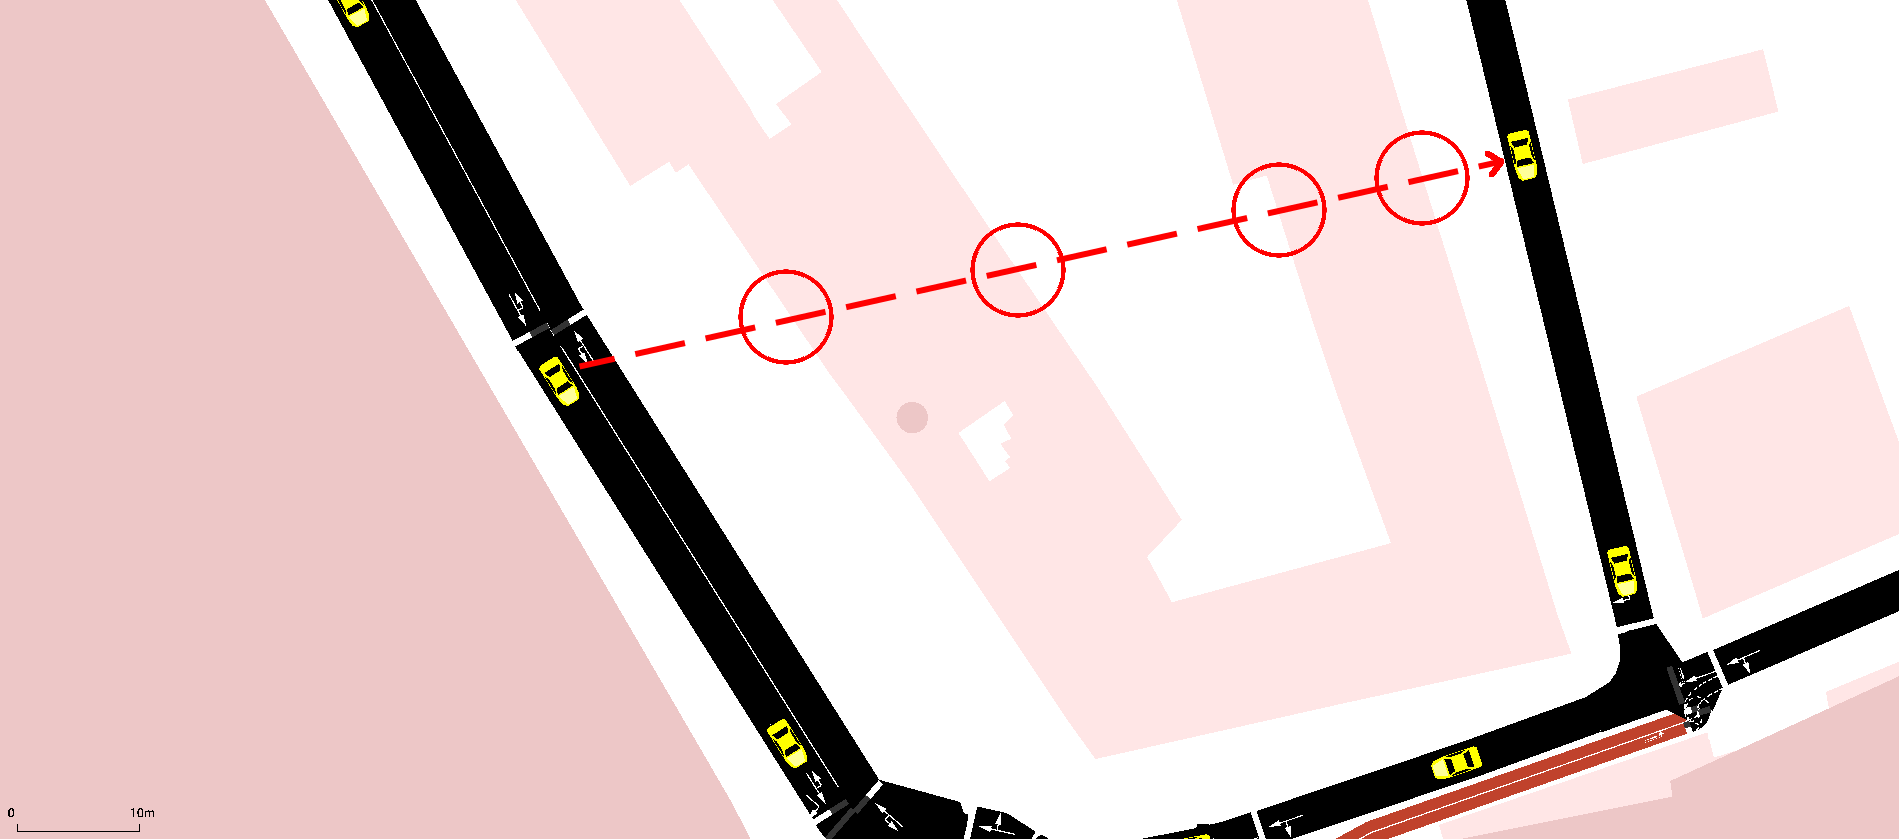
\includegraphics[width=\textwidth]{immagini/sumo-obstacle}
			\caption{Example of obstacle shadowing in vehicle-to-vehicle communication. Walls encountered by the signal are surrounded in red circles}
			\label{fig:sumo-obstacle}
		\end{figure}
%
%%**************************************************************
%\chapter{L'azienda}
%\label{cap:lazienda}
%%**************************************************************
%
%%Introduzione al contesto applicativo.\\
%
%%\noindent Esempio di utilizzo di un termine nel glossario \\
%%\gls{api}. \\
%
%%\noindent Esempio di citazione in linea \\
%%\cite{site:agile-manifesto}. \\
%%
%%\noindent Esempio di citazione nel pie' di pagina \\
%%citazione\footcite{womak:lean-thinking} \\
%
%%**************************************************************
%\section{Contesto aziendale}
%
%	IBC è nata nel 1980 come concessionaria \gls{NCR}. Le sue prime attività per conto di NCR riguardavano la fornitura di attrezzature \textit{hardware} per i punti vendita, come ad esempio \gls{POS} e \textit{scanner}. Successivamente, essa si è specializzata nella produzione di \textit{software} specifici per il mercato \gls{retail}, offrendo soluzioni personalizzate in base alle esigenze del singolo cliente.
%	
%	
%	Nel 1995 IBC fonda la sua sede a Peraga di Vigonza, in provincia di Padova. Ha sede tutt'ora nello stesso luogo, con tre filiali ad Alessandria, Trieste e Viterbo.
%	
%	\begin{figure}[H]
%		\centering
%		
\includegraphics[scale=0.7]{immagini/logo-ibc}
%		\caption{Logo IBC (\url{https://www.ibc.it/}).}
%	\end{figure}
%
%	\begin{figure}[H]
%		\centering
%		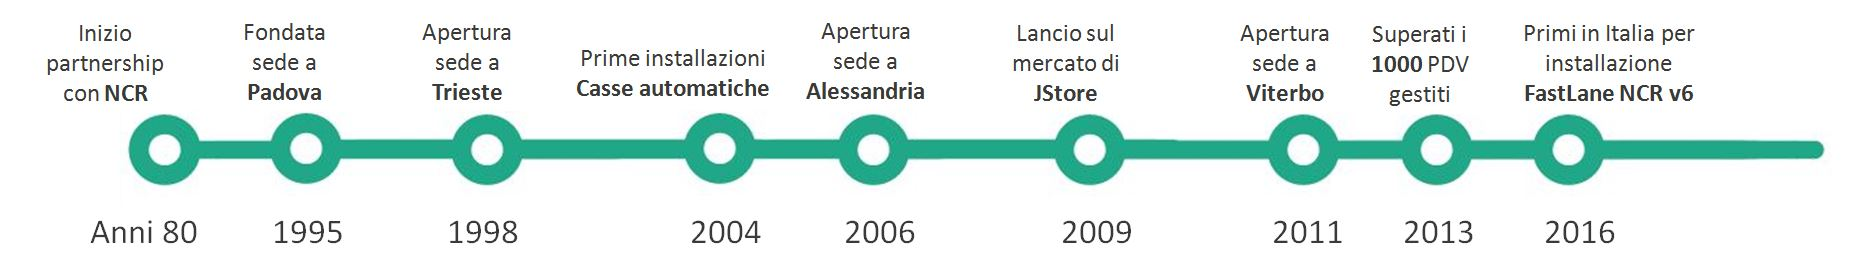
\includegraphics[width=\textwidth]{immagini/cronologia-ibc}
%		\caption{Cronologia IBC (\url{https://www.ibc.it/}).}
%	\end{figure}
%
%	IBC è stata una delle prime \textit{software house} italiane a realizzare progetti riguardanti la \gls{fidelity} e la profilazione dell'utente finale. Correntemente gestisce circa mille punti vendita, avendo installato quattromila casse e quattrocento postazioni \textit{self checkout}. 
%	
%	Attualmente, l'azienda opera principalmente su tre aree:
%	\begin{itemize}
%		\item \textbf{Sviluppo progetti}.
%		\item \textbf{Fornitura prodotti \textit{software} e \textit{hardware}}.
%		\item \textbf{Servizi e assistenza}.	
%	\end{itemize}
%	Fornirò spiegazioni ed esempi riguardo queste aree nelle sezioni successive di questo capitolo.
%	L'azienda possiede inoltre due certificazioni:
%	\begin{itemize}
%		\item \textbf{Certificazione di qualità UNI EN ISO 9001:2008:} per la commercializzazione e l'assistenza di misuratori fiscali, strumenti di pesatura, strumenti per l'automazione del punto vendita e POS bancari.
%		\item \label{laboratorio}
%		 \textbf{Certificazione per la verifica periodica dei misuratori fiscali:} IBC è abilitata alla verificazione periodica dei misuratori fiscali. Inoltre, è anche riconosciuta come laboratorio accreditato presso la CCIAA di Padova per le verifiche metriche degli strumenti di pesatura
%	\end{itemize}
%
%	Per fornire prodotti e servizi aggiornati, l'azienda collabora con vari \textit{partner} tecnologici, tra cui: NCR, Verifone, Motorola, Datalogic, Bizerba, Lenovo e Maind informatica.
%%	\begin{itemize}
%%		\item NCR.
%%		\item Verifone.
%%		\item Motorola.
%%		\item Datalogic.
%%		\item Bizerba.
%%		\item Lenovo.
%%		\item Maind informatica.
%%	\end{itemize}
%	
%	Inoltre, per garantire il servizio di assistenza, l'azienda intrattiene rapporti con: Master Office, InfoMaint, IT-Avantec, BSS, GAB Tamagnini.
%%	\begin{itemize}
%%		\item Master Office.
%%		\item InfoMaint.
%%		\item IT-Avantec.
%%		\item BSS.
%%		\item GAB Tamagnini.
%%	\end{itemize}
%
%	I clienti principali di IBC fanno tutti parte della \gls{GDO}. Tra di essi, troviamo sia clienti nazionali, come ad esempio il Gruppo UniComm, Benetton, Despar, Lando e Rossetto, sia internazionali, come ad esempio Würth Superstore.
%
%	\subsection{Prodotti}
%	I prodotti che IBC fornisce si dividono principalmente in due categorie:
%	\begin{itemize}
%		\item \textit{Hardware}.
%		\item \textit{Software}.
%	\end{itemize}
%
%	\subsubsection*{\textit{Hardware}}
%	I prodotti \textit{hardware} sono costituiti principalmente da strumenti di cassa e di pagamento. L'azienda non produce direttamente questo tipo di prodotti, ma opera da distributore, installatore e manutentore.
%	
%	\begin{enumerate}
%		\item \textbf{Soluzioni \textit{self}:} prodotti che consentono al cliente di concludere la spesa ed effettuare il pagamento autonomamente. Alcuni esempi di questa tipologia di prodotti sono le casse NCR Fastlane Selfserv Checkout Versione 6 (a sinistra nell'immagine) e i Kiosk NCR Selfserv 85 (a destra).
%	
%
%		\begin{figure}[H]
%		\centering
%		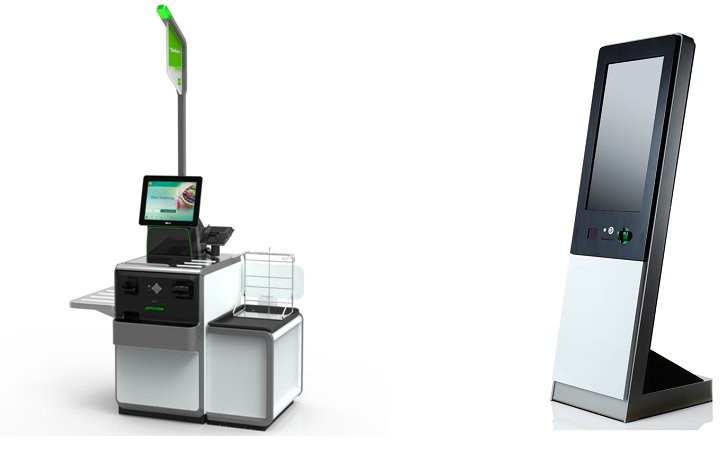
\includegraphics[scale=0.45]{immagini/soluzioni-self}
%		\caption{Soluzioni \textit{self} (\url{https://www.ibc.it/}).}
%		\end{figure}
%	
%		\item \textbf{Soluzioni POS:} si tratta di terminali che permettono al cliente di pagare utilizzando carte di credito, di debito o prepagate.
%	
%		\item \textbf{Periferiche:} \textit{scanner}, stampanti, \textit{monitor} e tutte le altre periferiche per aggiungere funzionalità ai POS e snellire le operazioni di \textit{checkout}.
%		\begin{figure}[H]
%			\centering
%			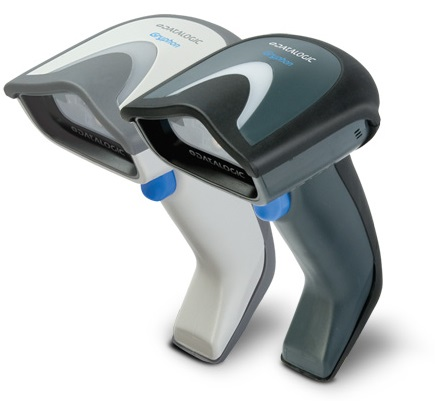
\includegraphics[scale=0.4]{immagini/periferiche}
%			\caption{\textit{Scanner} Datalogic Gryphon M4130 (\url{https://goo.gl/MZqts3}).}
%		\end{figure}
%	
%		\item \textbf{Terminali \textit{mobile}:} palmari che utilizzano sia Android che Windows, in modo da poter fornire compatibilità con la maggior parte dei sistemi dei clienti.
%		
%		\item \textbf{Terminali di pagamento:} strumenti (come ad esempio i PIN Pad) che permettono al cliente di inserire il numero della sua carta durante il pagamento. Garantiscono sicurezza e velocità durante l'esecuzione di questa operazione.
%		\begin{figure}[H]
%			\centering
%			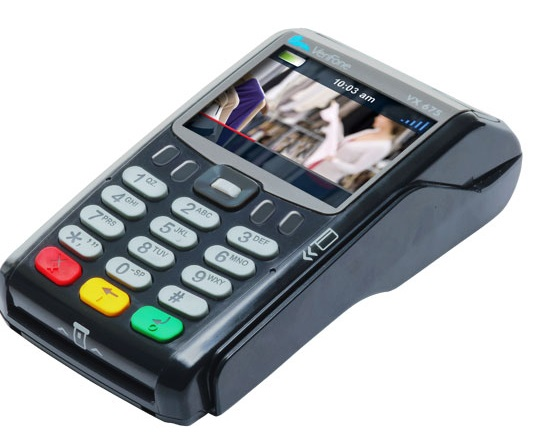
\includegraphics[scale=0.3]{immagini/terminali-di-pagamento}
%			\caption{Pin PAD Verifone VX675 (\url{https://www.ibc.it/}).}
%		\end{figure}
%	
%		\item \textbf{\textit{Server}:} prodotti da installare nei punti vendita. Essi riescono a gestire un elevato numero di richieste concorrenti, caratteristica fondamentale soprattutto nelle operazioni di gestione magazzino.
%		
%		\item \textbf{Bilance:} strumenti che garantiscono alta precisione nella pesatura. Sono inoltre programmabili, personalizzabili e integrabili allo \textit{scanner} per ampliare le funzionalità della postazione cassa. Sono anche utilizzate nella maggior parte dei reparti ortofrutta, permettendo al cliente di effettuare le operazioni di pesatura autonomamente.
%		
%		\begin{figure}[H]
%			\centering
%			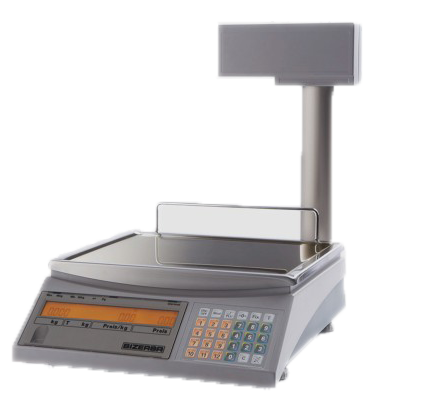
\includegraphics[scale=0.4]{immagini/bilance}
%			\caption{Bilancia Bizerba EC 100 (\url{https://goo.gl/dhTc9F}).}
%		\end{figure}
%	
%	\end{enumerate}
%
%	\subsubsection*{\textit{Software}}
%	
%	Oltre a fornire \textit{hardware}, IBC produce anche \textit{software}. Solitamente i clienti richiedono la realizzazione di soluzioni personalizzate. Per far ciò, l'azienda si è dotata di soluzioni modulari e flessibili.
%	
%	\begin{enumerate}
%		\item \textbf{JStore:} questo \textit{software} è una \textit{suite} completa che offre servizi per gli ambienti \textit{retail}. JStore, una volta installato in sede, permette la gestione e il controllo di tutti i punti vendita. Una delle caratteristiche principali di questo \textit{software} è la sua modularità, in modo da poter essere ampliato e modificato senza intaccare le altre funzionalità. JStore è realizzato in linguaggio Java, quindi è particolarmente adatto ad ambienti multipiattaforma.
%		\begin{figure}[H]
%			\centering
%			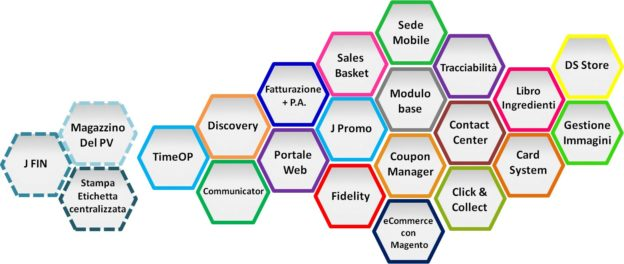
\includegraphics[scale=1.0]{immagini/jstore-moduli}
%			\caption{Moduli JStore (\url{https://www.ibc.it/}).}
%		\end{figure}
%		
%		La \textit{suite} copre quattro aree strategiche principali. Ogni area utilizza vari moduli per fornire le funzionalità necessarie.
%		\begin{enumerate}
%			\item \textbf{\textit{E-commerce}:} la prima area è dedicata agli acquisti via \textit{web}, sia di tipo classico (ovvero dalla creazione dell'ordine \textit{online} fino alla consegna), sia di tipo \gls{clickandcollect}.
%			Quest'area fa utilizzo di due moduli:
%			\begin{figure}[H]
%				\centering
%				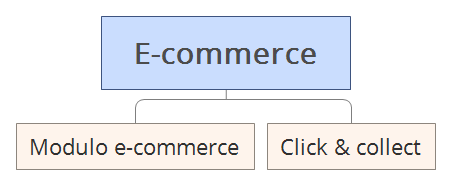
\includegraphics[scale=0.3]{immagini/e-commerce}
%				\caption{Moduli area \textit{e-commerce}}
%			\end{figure}
%		
%			\begin{itemize}
%				\item \textbf{Modulo \textit{e-commerce}:} questo modulo sfrutta un'integrazione della piattaforma di \textit{content management} Magento che gestisce la parte di logistica, preparazione dell'ordine e organizzazione della spedizione integrata con il magazzino.
%				\item \textbf{Modulo \textit{click \& collect}}: si integra con il sistema centrale per la divulgazione anagrafiche e prezzi del cliente, e con gli altri moduli di JStore per la gestione di \textit{fidelity}, \textit{coupon}, promozioni e fatturazione. Il modulo supporta anche \textit{tablet} e \gls{pda}. Inoltre, fornisce funzionalità multispesa (l'operatore può preparare contemporaneamente più spese) e multioperatore (più operatori possono preparare contemporaneamente la stessa spesa).
%			\end{itemize}
%			
%			\item \textbf{\textit{Marketing}:} la seconda area è dedicata alla gestione delle promozioni e dei \textit{coupon}. I moduli di quest'area si occupano di monitorare il flusso di informazioni, generare reportistica e tenere traccia dei \textit{coupon} durante tutti i passaggi di stato.
%			\begin{figure}[H]
%				\centering
%				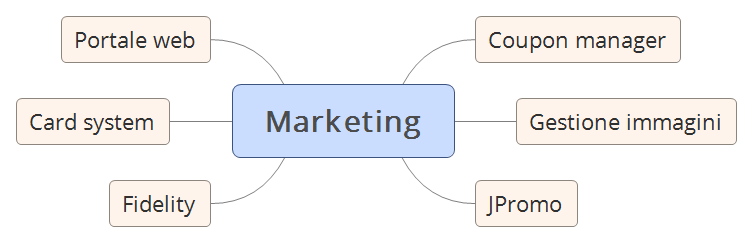
\includegraphics[scale=0.3]{immagini/marketing}
%				\caption{Moduli area marketing}
%			\end{figure}
%		
%			\begin{itemize}
%				\item \textbf{Modulo \textit{coupon manager}:} permette la gestione e la definizione di caratteristiche di valore, fruizione e validità dei buoni spesa.
%				\item \textbf{Modulo gestione immagini:} permette di pubblicare le immagini nei formati richiesti, effettuando il \textit{resize} automatico dell'immagine.
%				\item \textbf{Modulo JPromo:} il modulo si occupa della gestione delle promozioni di negozio. Se utilizzato in ambiente centralizzato, permette di generare un pacchetto promozioni di un'intera catena di negozi.
%				\item \textbf{Modulo \textit{fidelity}:} gestisce in modo centralizzato le funzionalità relative alle carte fedeltà, come ad esempio accumulo e utilizzo punti e ritiri dei premi.
%				\item \textbf{Modulo \textit{card system}:} piattaforma \textit{web} che permette di amministrare le \textit{gift card}.
%				\item \textbf{Modulo portale \textit{web}:} modulo che fornisce un canale di comunicazione tra il punto vendita e il cliente fidelizzato, offrendo varie informazioni su promozioni e saldo punti.
%			\end{itemize}
%		
%		\item \textbf{Gestione operativa del punto vendita:} la terza area soddisfa le esigenze di negozio, dalla fatturazione, la tracciabilità e l'inventario fino alla gestione delle comunicazioni con i clienti.
%		
%		\begin{figure}[H]
%			\centering
%			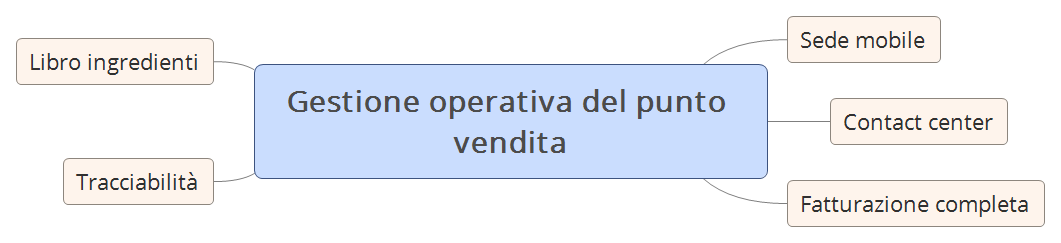
\includegraphics[scale=0.3]{immagini/gestione-operativa}
%			\caption{Moduli gestione operativa del punto vendita}
%		\end{figure}
%		
%		\begin{itemize}
%			\item \textbf{Modulo sede \textit{mobile}:} modulo che gestisce in modo centralizzato l'inventario permanente dei dispositivi mobili.
%			\item \textbf{Modulo \textit{contact center}:} piattaforma \textit{web} in grado di gestire la registrazione delle richieste (come ad esempio i reclami dei clienti), le soluzioni proposte e le risposte dei clienti.
%			\item \textbf{Modulo fatturazione completa:} permette la rilevazione di fatture e scontrini emessi nei punti vendita. Inoltre, supporta l'invio automatico ad intervalli regolari e personalizzabili degli scontrini dal punto vendita alla sede.
%			\item \textbf{Modulo tracciabilità:} modulo che gestisce la tracciabilità dei lotti carne e ittici nei punti vendita.
%			\item \textbf{Modulo libro ingredienti:} il modulo permette di memorizzare e riconoscere gli allergeni presenti all'interno dei prodotti. Questa funzionalità consente la pubblicazione del libro degli ingredienti secondo le normative europee.
%		\end{itemize}
%	
%		\item \textbf{Gestione strategica e di monitoraggio:} la quarta e ultima area comprende tutti i moduli che riguardano l'osservazione e il controllo dei sistemi e delle informazioni. Lo scopo di quest'area è definire le strategie di gestione, come la produttività del lavoro dei cassieri e i dati del venduto.
%		
%		\begin{figure}[H]
%			\centering
%			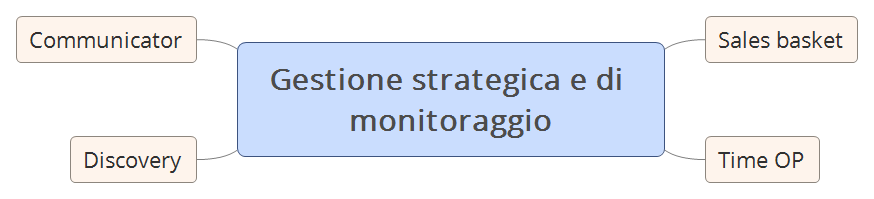
\includegraphics[scale=0.3]{immagini/gestione-strategica}
%			\caption{Moduli gestione strategica e di monitoraggio}
%		\end{figure}
%		
%		\begin{itemize}
%			\item \textbf{Modulo \textit{sales basket}:} strumento che permette di analizzare le informazioni sul venduto a partire dagli scontrini. Supporta l'attivazione di \textit{alert} in base a eventi, con la possibilità di inviare messaggi via SMS o \textit{e-mail}.
%			\item \textbf{Modulo \textit{time OP}:} modulo che permette l'analisi delle casse, fornendo dati sulla produttività del lavoro dei cassieri e consentendo di effettuare comparazioni tra i punti vendita della catena.
%			\item \textbf{Modulo \textit{discovery}:} si occupa di monitorare e recuperare le informazioni tecniche e di stato dei sistemi, inviando segnalazioni di errori quando necessario.
%			\item \textbf{Modulo \textit{communicator}:} modulo per la gestione e il monitoraggio della divulgazione di informazioni in JStore.
%		\end{itemize}
%	
%		\end{enumerate}
%
%
%		\item \textbf{i\_STORE:} \textit{software} di \gls{backoffice} che permette di gestire dalla sede le principali esigenze dei punti vendita. È particolarmente adatto alle aziende del settore distributivo, dato il \textit{focus} sulla movimentazione delle merci. Uno dei vantaggi principali di i\_STORE è il funzionamento in modo indipendente rispetto ai modelli di casse e bilance installate nel punto vendita.
%			
%		\begin{figure}[H]
%			\centering
%			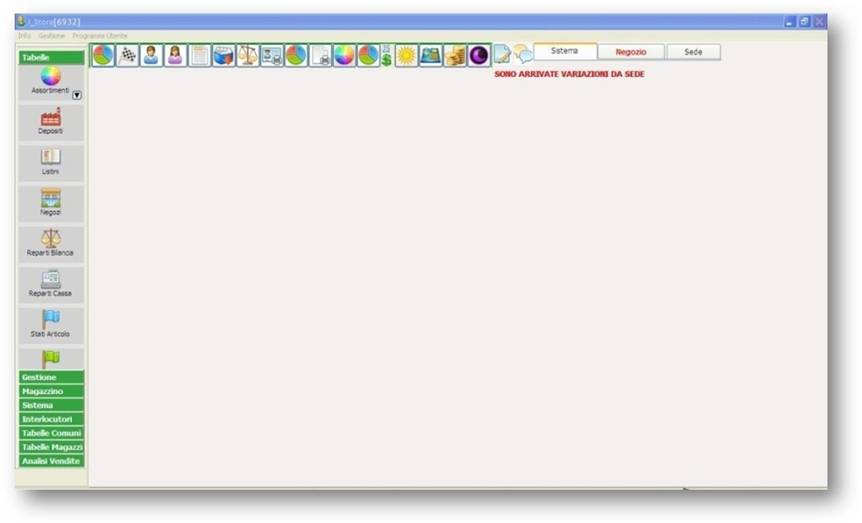
\includegraphics[scale=0.4]{immagini/i-store}
%			\caption{\textit{Screenshot} di i\_STORE (\url{https://www.ibc.it/}).}
%		\end{figure}
%	
%		\item \textbf{ARS:} \textit{software} realizzato da NCR e installato da IBC. Questo \textit{software} è installato su casse tradizionali e \textit{self-checkout}, indipendentemente dall'\textit{hardware} e dal sistema operativo. Gestisce l'applicazione delle logiche promozionali durante la vendita e il pagamento.
%		
%		\item \textbf{UPB:} \textit{software} NCR che permette alle casse di offrire vari servizi, come il pagamento di utenze, tasse di abilitazione di carte prepagate e la possibilità di effettuare ricariche telefoniche. Con questo \textit{software} è possibile portare a termine, durante il pagamento in cassa, qualsiasi attività che tipicamente viene svolta dalla tabaccheria o dalle poste.
%		
%		\item \textbf{WinEPTS}: è un \textit{software} NCR per i pagamenti elettronici che consente al \textit{retailer} di rendersi completamente autonomo dalle banche, diminuendo (e in alcuni casi azzerando) le commissioni sui pagamenti effettuati tramite bancomat.
%		
%		\item \textbf{Customer Point:} soluzione IBC installata su Kiosk per permettere al cliente di avere informazioni su prodotti e servizi. Il \textit{software} è anche integrabile su dispositivi \textit{touch}.
%		
%		\begin{figure}[H]
%			\centering
%			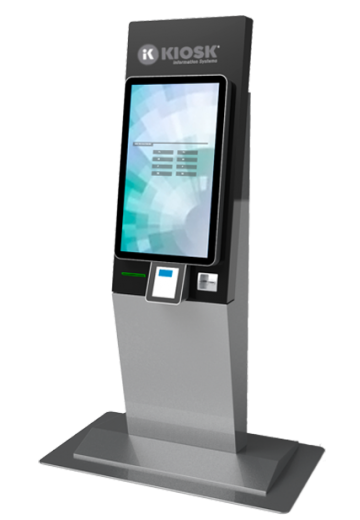
\includegraphics[scale=0.4]{immagini/kiosk}
%			\caption{Un Kiosk (\url{https://goo.gl/PhTxdc}).}
%		\end{figure}
%		
%		\item \textbf{MobileStore:} \textit{app mobile} per la raccolta remota dei dati del punto vendita. Supporta la lettura dei codici a barre e la memorizzazione di informazioni, effettuandone anche una prima elaborazione direttamente sul terminale.
%		
%		\item \textbf{Libro guida ordini:} \textit{app mobile} disponibile su \textit{tablet} che permette il riordino degli articoli in maniera digitale, sostituendo il tradizionale libro cartaceo ed eliminandone i costi di gestione.
%		
%		\item \textbf{Assistente di negozio:} \textit{app mobile} mirata a dare supporto al cliente nella vendita \textit{no food}. Il \textit{software} permette di dare informazioni e caratteristiche tecniche dei prodotti accedendo direttamente all'anagrafica di sede.
%		
%		\item \textbf{Fidelity:} \textit{app mobile} per la gestione delle carte fedeltà rivolta al cliente. L'installazione dell'applicazione è semplificata in quanto è possibile installarla rilevando direttamente il QR \textit{code}. Attraverso l'\textit{app} il cliente può compiere varie operazioni, come ad esempio prenotare la spesa, gestire i \textit{coupon} e visualizzare gli scontrini.
%		
%		\item \textbf{Yourself:} \textit{app} installabile sui lettori portatili in grado di scannerizzare i codici a barre dei prodotti, in modo da velocizzare il pagamento in cassa. Collegandosi a JStore, l'applicazione permette al cliente di evitare la fila alle casse, offrendogli la possibilità di imbustare direttamente la spesa.
%	\end{enumerate}
%	
%	\subsection{Servizi}
%		Nel mercato odierno, i prodotti non sono l'unica caratteristica che permette ad un'azienda di aver successo. Data la collaborazione, in molti casi pluriennale, tra IBC e i suoi clienti, l'azienda fornisce vari servizi. 
%		
%		\begin{enumerate}
%			\item \textbf{Assistenza:} IBC fornisce assistenza \textit{software} e \textit{hardware} attraverso servizi di \textit{call center}, \textit{help desk} e interventi \textit{on-site}. Una delle caratteristiche di forza dell'assistenza IBC è la gestione delle segnalazioni in tempi brevi e garantiti. Per garantire ciò, l'azienda rimane aperta quasi tutto l'anno, compresi i \textit{weekend}. 
%			
%			\begin{figure}[H]
%				\centering
%				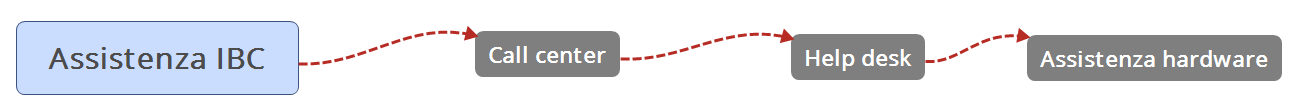
\includegraphics[width=\textwidth]{immagini/assistenza}
%				\caption{Percorso assistenza IBC.}
%			\end{figure}
%		
%			Una richiesta di assistenza a IBC attraversa vari stadi:
%			\begin{enumerate}
%				\item \textbf{\textit{Call center}:} riceve e registra le richieste di assistenza, indicandone l'urgenza e assegnando un codice identificativo. Successivamente, inoltra la chiamata ai tecnici di \textit{help desk}.
%				\item \textbf{\textit{Help desk}:} analizza il problema tecnico dichiarato e fornisce una soluzione per via telefonica. Nel caso la soluzione non sia efficace o l'\textit{help desk} non abbia strumenti o competenze sufficienti, quest'ultimo assegna la risoluzione della segnalazione al reparto IBC più adatto.
%				\item \textbf{Assistenza \textit{hardware}:} qualora il problema segnalato sia di natura \textit{hardware}, il personale incaricato provvede ad effettuare le operazioni di manutenzione necessarie e ripristina le normali condizioni di funzionamento presso la sede del cliente.
%			\end{enumerate}
%			
%			\item \textbf{Laboratorio metrologico:} come descritto in \ref{laboratorio}, IBC è anche laboratorio accreditato presso la CCIAA di Padova per le verifiche metriche degli strumenti di pesatura. I servizi offerti riguardano la verifica periodica prevista per legge di bilance e strumenti per la pesatura, sia automatici che non. La verifica, oltre che alla scadenza, è obbligatoria anche dopo un'attività di manutenzione che ha rimosso i sigilli dallo strumento.
%			
%			
%			In aggiunta ai servizi previsti per legge da un laboratorio metrologico, IBC offre in aggiunta servizi ulteriori, come ad esempio il trasporto delle masse necessarie per effettuare le prove, la conservazione dei dati presso l'archivio aziendale e la gestione automatica della periodicità delle scadenze. Inoltre, per legare il servizio di assistenza al servizio di laboratorio, nel caso di bilance che non risultino idonee alla verifica periodica, IBC offre gratuitamente la seconda uscita dell'ispettore metrico per l'intervento di riparazione. 
%		\end{enumerate}
%		
%\section{Organizzazione aziendale}
%	\subsection{Organizzazione e reparti}
%		IBC, internamente, è divisa in due macro aree:
%		\begin{itemize}
%			\item \textbf{Amministrativa:} area che comprende le funzioni aziendali di amministrazione, risorse umane, organizzazione e finanza.
%			\item \textbf{Prodotti e assistenza}: area che comprende lo sviluppo di prodotti, principalmente \textit{software}, e l'assistenza post vendita.
%		\end{itemize}
%		
%		Essendo stato collocato all'interno del team Java 3 per lo svolgimento dello \textit{stage}, ho potuto comprendere meglio il funzionamento dell'area prodotti e assistenza. Per questo motivo mi concentrerò maggiormente sull'analisi di quest'area. In aggiunta a ciò, ho avuto rapporti molto limitati con l'area amministrativa, per cui non sono in grado di fare un'analisi approfondita del funzionamento interno di quest'ultima.
%		
%		L'area prodotti e assistenza è suddivisa in vari reparti:
%		\begin{itemize}
%			\item \textbf{Reparto Analisi:} reparto che si occupa di comprendere le necessità dei clienti e formulare un'analisi comprensibile dal personale tecnico aziendale. Gli analisti sono il primo passo verso la formulazione di una soluzione \textit{software}. Questo reparto opera sia presso il cliente che presso la sede IBC.
%			\item \textbf{Reparto Sviluppo:} reparto che si occupa della realizzazione effettiva del prodotto finale, utilizzando varie tecnologie e linguaggi di programmazione. Il reparto sviluppo è composto da:
%			\begin{itemize}
%				\item Tre \textit{team} Java, che si occupano della realizzazione di \textit{web app} e dello sviluppo di JStore.
%				\item Un \textit{team} \textit{device}, le cui mansioni sono la realizzazione e la manutenzione delle applicazioni \textit{mobile}.
%				\item Un \textit{team} che si occupa della realizzazione e manutenzione del \textit{software} delle casse.
%			\end{itemize}
%			\item \textbf{Reparto \textit{Customer Care} e \textit{Help Desk}}: reparto che si occupa dell'assistenza post vendita, sia su prodotti \textit{hardware} che \textit{software}. Ho potuto notare che molte segnalazioni di natura \textit{software} vengono fatte risolvere al reparto sviluppo, spesso provocando ritardi in altre attività.
%		\end{itemize}
%		Nell'elenco mancano reparti come Ricerca e Sviluppo e reparti che si occupano di progettazione. Questa mancanza è dovuta al fatto che IBC non ha dei reparti dedicati per questi scopi, ma si affida a singoli dipendenti (o in ogni caso gruppi molto ristretti) che non costituiscono reparti a sé stanti. Ho potuto notare questa propensione anche in relazione al mio \textit{stage}: per l'azienda, le attività da me svolte rientrano nella funzione ricerca e sviluppo. Fornirò maggiori informazioni su questo punto, insieme ad altri obiettivi aziendali legati agli \textit{stage}, nel capitolo \ref{cap:loffertadistage}.
%		
%		
%		La tendenza nel far prendere decisioni importanti ad un numero ristretto di persone si sposa con la struttura aziendale che ho potuto rilevare. Anche se giuridicamente IBC si presenta come una S.r.l.,  nella pratica il suo funzionamento è quello di un'impresa a conduzione familiare, data la consanguineità dei ruoli di più alto livello.
%		 
%		Tra i vantaggi di questo approccio ho potuto notare la facilità nel prendere decisioni anche importanti in tempi relativamente brevi. Se le stesse decisioni avessero dovuto attraversare vari organi aziendali prima di essere prese, sicuramente sarebbe passato molto più tempo e alcune avrebbero riportato una perdita di efficacia.
%		Gli svantaggi principali sono invece: 
%		\begin{itemize}
%			\item Troppe libertà e responsabilità lasciate al personale tecnico, specialmente ai programmatori. Data la mancanza di un reparto che si occupa di progettazione di dettaglio, il programmatore ha troppa libertà decisionale su come implementare la soluzione che gli viene assegnata. Alcune volte ho potuto notare come decisioni prese da un programmatore abbiano causato incomprensioni e ritardi nelle attività di altri \textit{team} di sviluppo.
%			\item Ritardi e impossibilità nel prendere decisioni di natura architetturale quando anche soltanto uno dei (pochi) dipendenti che si occupa di progettazione è assente.
%		\end{itemize}
%	
%	\subsection{Processi}
%		Il modello di sviluppo che IBC ha adottato si rifà ai principi del modello Agile, consultabili al seguente indirizzo:
%		\begin{center}
%			\url{http://agilemanifesto.org/iso/it/principles.html}
%		\end{center}
%		
%		\begin{figure}[H]
%			\centering
%			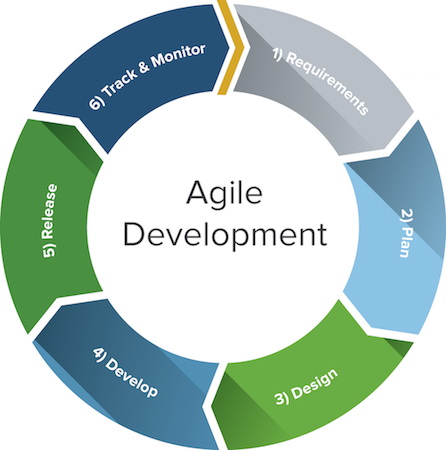
\includegraphics[scale=0.4]{immagini/ciclo-agile}
%			\caption{Ciclo di sviluppo Agile (\url{https://goo.gl/ESua3X}).}
%		\end{figure}
%		
%		I principi che ho percepito come i più seguiti sono:
%		\begin{itemize}
%			\item \jquote{Committenti e sviluppatori devono lavorare insieme
%			quotidianamente per tutta la durata del progetto}. Ho constatato che il personale tecnico di alcuni clienti di IBC ha contatti quotidiani con i programmatori dell'azienda, fino ad arrivare ad influenzare il modo con cui le funzionalità sono implementate.
%			\item \jquote{Una conversazione faccia a faccia è il modo più efficiente e più efficace per comunicare con il \textit{team} ed all'interno del \textit{team}}. Nonostante l'utilizzo di \textit{software} di \textit{ticketing} e la presenza di procedure ben definite per il contatto tra membri di \textit{team} diversi, il personale predilige un rapporto faccia a faccia la maggior parte delle volte. In molti casi ho potuto rilevare che problemi di incomprensioni tra sviluppatori sono stati risolti in modo molto efficace semplicemente parlando di persona.
%		\end{itemize}
%		
%		Tuttavia, IBC non segue i principi alla lettera, ma adatta le sue reazioni a seconda del caso. Ad esempio, l'azienda non accetta cambiamenti sostanziali nei requisiti anche a stadi avanzati dello sviluppo. Nel caso in cui ciò avvenisse, il cliente dovrebbe pagare una somma di denaro per finanziare le ore aggiuntive necessarie a sviluppare (o modificare) il \textit{software} in modo che copra le nuove richieste. Personalmente sono d'accordo con questa linea di pensiero.
%		
%		
%		Un altro punto di distacco tra il modello adottato da IBC e Agile sono le riunioni. Contrariamente alla prassi adottata dal modello Agile, ovvero riunioni giornaliere (\textit{Daily standup meeting}), IBC tiene riunioni settimanali. 
%		
%		
%		Tenendo conto di questi (e altri) punti, ho potuto percepire che l'azienda non adotta ciecamente il modello Agile, ma ne sfrutta solamente i punti di forza, tralasciando completamente le \jquote{cerimonie} che la metodologia è solita portare con sé. 
%		
%		
%		
%	\subsection{Progetti}
%		Il lavoro all'interno dell'azienda è organizzato a progetti. Ogni \textit{team} si trova a lavorare contemporaneamente a più progetti, richiedendo un cambio di contesto a volte molto rapido. 
%		
%		
%		 Per quanto riguarda il \textit{team} Java con cui ho lavorato a più stretto contatto, ho potuto notare che, oltre ai progetti, il \textit{team} doveva gestire anche l'infrastruttura e alcuni moduli di JStore. Nonostante la differenziazione dei \textit{task} assegnati e i molti ambiti gestiti, i membri del gruppo hanno quasi sempre gestito il lavoro in modo organizzato. Questo denota una buona organizzazione all'interno del \textit{team}.
%		 Talvolta, più \textit{team} hanno dovuto lavorare su moduli differenti dello stesso progetto e anche in quei casi la comunicazione si è dimostrata efficace.
%		 
%		
%\section{Tecnologie a supporto dei processi}
%	\begin{figure}[H]
%		\centering
%		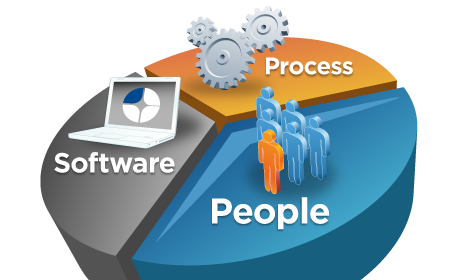
\includegraphics[scale=0.4]{immagini/tecnologie-processi}
%		\caption{Persone, processi e tecnologie (\url{https://goo.gl/KX59QR}).}
%	\end{figure}
%	Con l'aumentare delle dimensioni di un'azienda, quest'ultima ha sempre più bisogno di tecnologie che supportino i processi. Infatti, nonostante le persone siano una parte fondamentale per il raggiungimento degli obiettivi aziendali, le tecnologie aiutano sia a rendere il raggiungimento di tali obiettivi ripetibile sia a contenere i costi.
%	
%	\subsection{Gestione di progetto}
%		\subsubsection*{SysAid}
%			\begin{figure}[H]
%				\centering
%				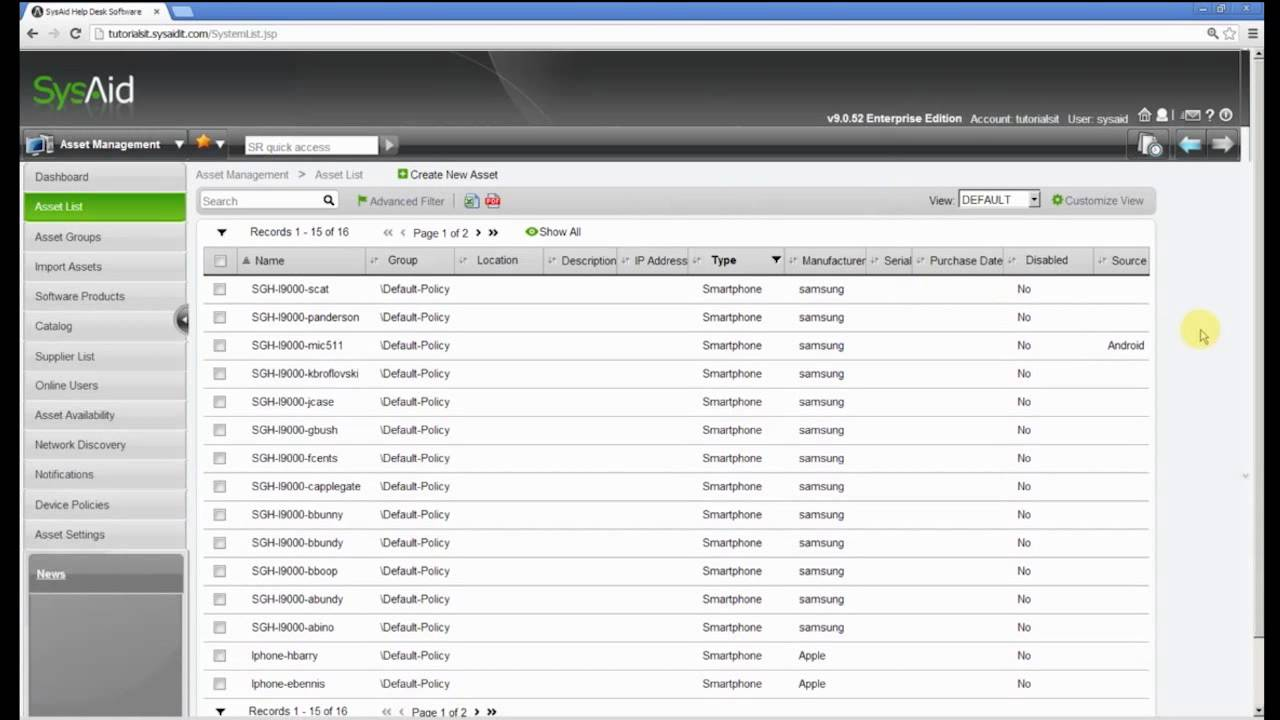
\includegraphics[width=\textwidth]{immagini/sysaid}
%				\caption{\textit{Screenshot} di SysAid (\url{https://goo.gl/cACkfo}).}
%			\end{figure}
%			Il principale strumento adottato da IBC per la gestione di progetto è SysAid. SysAid è un \textit{software} di \textit{help desk} completo, utilizzato in quasi ogni reparto IBC. Questo \textit{software} offre varie funzionalità ed è integrabile anche su dispositivi \textit{mobile}. Ecco un elenco delle sue principali caratteristiche:
%			\begin{itemize}
%				\item \textbf{Gestione \textit{ticket}:} SysAid permette di inserire \textit{ticket} e di chiuderli una volta risolti. Questa funzionalità permette al reparto sviluppo di IBC di ricevere \textit{ticket} direttamente dal reparto \textit{customer care} e \textit{help desk} e di risolverli in autonomia, qualora non ci siano incomprensioni o problemi più gravi.
%				Il \textit{software} fornisce anche funzionalità di notifica e di regolazione delle priorità.
%				\item \textbf{Gestione \textit{asset}:} funzionalità che permette di rilevare automaticamente e gestire i dispositivi collegati alla rete aziendale.
%				\item \textbf{\textit{Knowledge base}:} permette di memorizzare documentazione e guide che consentono la risoluzione dei problemi più frequenti.
%				\item \textbf{Gestione \textit{dashboard}:} SysAid offre un rapporto in tempo reale dello stato dei \textit{ticket} e permette di avere \textit{report} di vario genere.
%			\end{itemize}
%
%	\subsection{Gestione della configurazione e versionamento}
%		\label{sec:configurazione}
%		\subsubsection*{SVN}
%			\begin{figure}[H]
%				\centering
%				
\includegraphics[scale=2.0]{immagini/svn}
%				\caption{Gestione centralizzata di SVN (\url{https://goo.gl/67AyyR}).}
%			\end{figure}
%		
%				Il sistema di versionamento utilizzato da IBC è Subversion (d'ora in poi SVN). Questo sistema offre un \textit{repository} centralizzato su cui gli sviluppatori effettuano dei \textit{commit} per pubblicare i cambiamenti da loro prodotti.
%				Alcune caratteristiche di SVN sono:
%				\begin{itemize}
%					\item L'atomicità dei \textit{commit}: qualora un \textit{commit} dovesse essere interrotto, il \textit{repository} non verrebbe lasciato in uno stato di inconsistenza.
%					\item Un'efficiente gestione dei \textit{file} binari.
%					\item Il \textit{branching} è un'operazione che richiede un tempo indipendente dalla dimensione dei dati.
%					\item La licenza è \gls{opensource}.
%				\end{itemize}
%				La centralizzazione di SVN, la caratteristica principale che garantisce la sua semplicità rispetto a soluzioni distribuite come Git, è anche il suo principale svantaggio. Infatti, in caso di impossibilità di accesso al \textit{repository}, è impossibile effettuare \textit{commit} e la gran parte delle funzionalità di versionamento è inutilizzabile. IBC sopperisce a questo rischio fornendo una connessione \textit{internet} affidabile all'interno dei propri stabili.
%				
%		\subsubsection*{Maven}
%			Apache Maven è un \textit{software} utilizzato per la gestione della configurazione e delle dipendenze tra un progetto e librerie esterne. In IBC viene utilizzato per gestire i progetti Java, anche se è possibile configurarlo per altri linguaggi.
%			Alla base di Maven c'è il POM (Project Object Model), ovvero un \textit{file} XML che descrive le \textit{directory} di progetto, le dipendenze e definisce come deve avvenire il processo di \textit{build}. Il \textit{download} delle dipendenze è gestito in modo automatico, tipicamente appoggiandosi ad un \textit{repository} centralizzato.
%			
%	\subsection{Sviluppo}
%		\label{sec:sviluppo}
%		\subsubsection*{Wicket}
%			Apache Wicket è un \textit{framework} \textit{web} lato \textit{server} che utilizza Java per lo sviluppo di \textit{web app}. Il \textit{framework} fornisce un insieme di componenti grafiche pronte all'uso, che permettono un'alta produttività a discapito della personalizzazione. 
%			Wicket risulta essere adatto allo sviluppo di \textit{web app} per conto dei clienti di IBC. Infatti, la maggior parte delle funzionalità richieste dai clienti è già implementata e gestita dai componenti di Wicket, minimizzando lo sviluppo di componenti personalizzate. 
%		
%	\begin{table}[H]
%		\centering
%		\begin{tabularx}{\textwidth}{|X | X | X | X | X |}
%			\hline
%			\rowcolor{lightgray}
%			\textbf{Gestione di progetto} & \textbf{{Config.} e \mbox{versionamento}} &  \textbf{Sviluppo} &  \textbf{IDE} &  \textbf{Vari}  \\
%			\hline
%			SysAid & SVN & Java & Eclipse & LibreOffice \\
%			\hline
%			& Maven & C++ & Android Studio & Skype \\
%			\hline
%			& Ant & Wicket & & \\
%			\hline
%			& & Bootstrap & & \\
%			\hline
%			& & Hibernate & & \\
%			\hline
%		\end{tabularx}
%	\caption{Principali tecnologie utilizzate da IBC.}
%	\end{table}
%	
%\section{Rapporto con l'innovazione}
%	Negli ultimi anni, il mondo del \textit{retail} in Italia sta avanzando in termini tecnologici. Le casse automatiche sono sempre più diffuse all'interno dei punti vendita e, con l'espansione di supermercati e ipermercati, molti clienti sentono la necessità di avere servizi aggiuntivi, come le ricariche telefoniche o i servizi tipici delle tabaccherie. 
%	
%	
%	IBC, per poter fornire soluzioni adatte alle richieste del mercato e dei clienti, necessita di stare al passo dal punto di vista tecnologico. Questo è il motivo per cui intrattiene rapporti con alcuni dei fornitori che offrono tecnologie più avanzate, come ad esempio NCR e Motorola. Queste collaborazioni permettono la fornitura e la manutenzione di \textit{hardware} sempre aggiornato.
%	
%	
%	Anche lo sviluppo di soluzioni multipiattaforma è uno dei punti di forza dell'azienda. Per poter soddisfare le richieste dei clienti, IBC offre soluzioni sia \textit{desktop} che \textit{mobile} compatibili con tutte le principali piattaforme. L'efficacia nello sviluppo di queste soluzioni multipiattaforma è data dall'utilizzo di linguaggi di programmazione come Java, particolarmente adatto a questo caso d'uso.
%	
%	
%	Dal punto di vista dei \textit{framework} e delle librerie adottate, l'azienda ha recentemente adottato Apache Wicket che, nonostante sia un \textit{framework} abbastanza vecchio, continua ad essere aggiornato e ad avere un discreto supporto.
%	
%	L'architettura alla base del prodotto principale di IBC, JStore, è basata su \gls{webservice} per garantire modularità ed interoperabilità. A mio avviso, una scelta architetturale di questo genere è matura e rivolta al futuro, in modo da abbandonare le architetture monolitiche del passato.
%	
%	
%	Una caratteristica negativa dal punto di vista dell'innovazione è la mancanza di implementazione ed esecuzione di \textit{test} automatici. Infatti, IBC non sfrutta alcun tipo di \textit{test} automatico per verificare o validare i \textit{software} prodotti. A mio avviso, una delle conseguenze più gravi di questa mancanza è la regressione, ovvero la possibilità di introdurre errori in \textit{software} precedentemente funzionante senza accorgersene immediatamente.
%	
%	
%	Ho assistito ad alcuni esempi di regressione durante la mia permanenza presso l'azienda. Ogni occasione ha portato all'impiego di numerose ore persona per risolvere i problemi introdotti. La maggior parte di queste situazione avrebbe potuto essere evitata sfruttando \textit{suite} di \textit{test} opportunamente configurate.
%	
%	
%
%%**************************************************************
%
%%**************************************************************
%%\section{Organizzazione aziendale}
%%
%%\begin{description}
%%    \item[{\hyperref[cap:processi-metodologie]{Il secondo capitolo}}] descrive ...
%%    
%%    \item[{\hyperref[cap:descrizione-stage]{Il terzo capitolo}}] approfondisce ...
%%    
%%    \item[{\hyperref[cap:analisi-requisiti]{Il quarto capitolo}}] approfondisce ...
%%    
%%    \item[{\hyperref[cap:progettazione-codifica]{Il quinto capitolo}}] approfondisce ...
%%    
%%    \item[{\hyperref[cap:verifica-validazione]{Il sesto capitolo}}] approfondisce ...
%%    
%%    \item[{\hyperref[cap:conclusioni]{Nel settimo capitolo}}] descrive ...
%%\end{description}
%%
%%Riguardo la stesura del testo, relativamente al documento sono state adottate le seguenti convenzioni tipografiche:
%%\begin{itemize}
%%	\item gli acronimi, le abbreviazioni e i termini ambigui o di uso non comune menzionati vengono definiti nel glossario, situato alla fine del presente documento;
%%	\item per la prima occorrenza dei termini riportati nel glossario viene utilizzata la seguente nomenclatura: \emph{parola}\glsfirstoccur;
%%	\item i termini in lingua straniera o facenti parti del gergo tecnico sono evidenziati con il carattere \emph{corsivo}.
%%\end{itemize}